\documentclass[
    xcolor={svgnames,dvipsnames},
    hyperref={colorlinks, citecolor=DeepPink4, linkcolor=DarkRed, urlcolor=DarkBlue}
    ]{beamer}  % for hardcopy add 'trans'

\mode<presentation>
{
  \usetheme{Singapore}
  % or ...
  \setbeamercovered{transparent}
  % or whatever (possibly just delete it)
}

\usefonttheme{professionalfonts}
%\usepackage[english]{babel}
% or whatever
%\usepackage[latin1]{inputenc}
% or whatever
%\usepackage{times}
%\usepackage[T1]{fontenc}
% Or whatever. Note that the encoding and the font should match. If T1
% does not look nice, try deleting the line with the fontenc.

%\usepackage{fontspec}
%\setmonofont{CMU Typewriter Text}
%\setmonofont{Consolas}

%%%%%%%%%%%%%%%%%%%%%% start my preamble %%%%%%%%%%%%%%%%%%%%%%

\addtobeamertemplate{navigation symbols}{}{%
    \usebeamerfont{footline}%
    \usebeamercolor[fg]{footline}%
    \hspace{1em}%
    \insertframenumber/\inserttotalframenumber
}


\usepackage{graphicx}
\usepackage{amsmath, amssymb, amsthm}
\usepackage{bbm}
\usepackage{mathrsfs}
\usepackage{xcolor}
\usepackage{fancyvrb}

% Quotes at start of chapters / sections
\usepackage{epigraph}  
%\renewcommand{\epigraphflush}{flushleft}
%\renewcommand{\sourceflush}{flushleft}
\renewcommand{\epigraphwidth}{6in}

%% Fonts

%\usepackage[T1]{fontenc}
\usepackage{mathpazo}
%\usepackage{fontspec}
%\defaultfontfeatures{Ligatures=TeX}
%\setsansfont[Scale=MatchLowercase]{DejaVu Sans}
%\setmonofont[Scale=MatchLowercase]{DejaVu Sans Mono}
%\setmathfont{Asana Math}
%\setmainfont{Optima}
%\setmathrm{Optima}
%\setboldmathrm[BoldFont={Optima ExtraBlack}]{Optima Bold}

% Some colors

\definecolor{aquamarine}{RGB}{69,139,116}
\definecolor{midnightblue}{RGB}{25,25,112}
\definecolor{darkslategrey}{RGB}{47,79,79}
\definecolor{darkorange4}{RGB}{139,90,0}
\definecolor{dogerblue}{RGB}{24,116,205}
\definecolor{blue2}{RGB}{0,0,238}
\definecolor{bg}{rgb}{0.95,0.95,0.95}
\definecolor{DarkOrange1}{RGB}{255,127,0}
\definecolor{ForestGreen}{RGB}{34,139,34}
\definecolor{DarkRed}{RGB}{139, 0, 0}
\definecolor{DarkBlue}{RGB}{0, 0, 139}
\definecolor{Blue}{RGB}{0, 0, 255}
\definecolor{Brown}{RGB}{165,42,42}


\setlength{\parskip}{1.5ex plus0.5ex minus0.5ex}

%\renewcommand{\baselinestretch}{1.05}
%\setlength{\parskip}{1.5ex plus0.5ex minus0.5ex}
%\setlength{\parindent}{0pt}

% Typesetting code
\definecolor{bg}{rgb}{0.95,0.95,0.95}
\usepackage{minted}
\setminted{mathescape, frame=lines, framesep=3mm}
\usemintedstyle{friendly}
%\newminted{python}{}
%\newminted{c}{mathescape,frame=lines,framesep=4mm,bgcolor=bg}
%\newminted{java}{mathescape,frame=lines,framesep=4mm,bgcolor=bg}
%\newminted{julia}{mathescape,frame=lines,framesep=4mm,bgcolor=bg}
%\newminted{ipython}{mathescape,frame=lines,framesep=4mm,bgcolor=bg}


\newcommand{\Fact}{\textcolor{Brown}{\bf Fact. }}
\newcommand{\Facts}{\textcolor{Brown}{\bf Facts }}
\newcommand{\keya}{\textcolor{turquois4}{\bf Key Idea. }}
\newcommand{\Factnodot}{\textcolor{Brown}{\bf Fact }}
\newcommand{\Eg}{\textcolor{ForestGreen}{Example. }}
\newcommand{\Egs}{\textcolor{ForestGreen}{Examples. }}
\newcommand{\Ex}{{\bf Ex. }}



\renewcommand{\theFancyVerbLine}{\sffamily
    \textcolor[rgb]{0.5,0.5,1.0}{\scriptsize {\arabic{FancyVerbLine}}}}

\newcommand{\navy}[1]{\textcolor{Blue}{\bf #1}}
\newcommand{\brown}[1]{\textcolor{Brown}{\sf #1}}
\newcommand{\green}[1]{\textcolor{ForestGreen}{\sf #1}}
\newcommand{\blue}[1]{\textcolor{Blue}{\sf #1}}
\newcommand{\navymth}[1]{\textcolor{Blue}{#1}}
\newcommand{\emp}[1]{\textcolor{DarkOrange1}{\bf #1}}
\newcommand{\red}[1]{\textcolor{Red}{\bf #1}}

% Symbols, redefines, etc.

\newcommand{\code}[1]{\texttt{#1}}

\newcommand{\argmax}{\operatornamewithlimits{argmax}}
\newcommand{\argmin}{\operatornamewithlimits{argmin}}

\DeclareMathOperator{\cl}{cl}
\DeclareMathOperator{\interior}{int}
\DeclareMathOperator{\Prob}{Prob}
\DeclareMathOperator{\determinant}{det}
\DeclareMathOperator{\trace}{trace}
\DeclareMathOperator{\Span}{span}
\DeclareMathOperator{\rank}{rank}
\DeclareMathOperator{\cov}{cov}
\DeclareMathOperator{\corr}{corr}
\DeclareMathOperator{\var}{var}
\DeclareMathOperator{\mse}{mse}
\DeclareMathOperator{\se}{se}
\DeclareMathOperator{\row}{row}
\DeclareMathOperator{\col}{col}
\DeclareMathOperator{\range}{rng}
\DeclareMathOperator{\dimension}{dim}
\DeclareMathOperator{\bias}{bias}


% mics short cuts and symbols
\newcommand{\st}{\ensuremath{\ \mathrm{s.t.}\ }}
\newcommand{\setntn}[2]{ \{ #1 : #2 \} }
\newcommand{\cf}[1]{ \lstinline|#1| }
\newcommand{\fore}{\therefore \quad}
\newcommand{\tod}{\stackrel { d } {\to} }
\newcommand{\toprob}{\stackrel { p } {\to} }
\newcommand{\toms}{\stackrel { ms } {\to} }
\newcommand{\eqdist}{\stackrel {\textrm{ \scriptsize{d} }} {=} }
\newcommand{\iidsim}{\stackrel {\textrm{ {\sc iid }}} {\sim} }
\newcommand{\1}{\mathbbm 1}
\newcommand{\dee}{\,{\rm d}}
\newcommand{\given}{\, | \,}
\newcommand{\la}{\langle}
\newcommand{\ra}{\rangle}

\newcommand{\boldA}{\mathbf A}
\newcommand{\boldB}{\mathbf B}
\newcommand{\boldC}{\mathbf C}
\newcommand{\boldD}{\mathbf D}
\newcommand{\boldM}{\mathbf M}
\newcommand{\boldP}{\mathbf P}
\newcommand{\boldQ}{\mathbf Q}
\newcommand{\boldI}{\mathbf I}
\newcommand{\boldX}{\mathbf X}
\newcommand{\boldY}{\mathbf Y}
\newcommand{\boldZ}{\mathbf Z}

\newcommand{\bSigmaX}{ {\boldsymbol \Sigma_{\hboldbeta}} }
\newcommand{\hbSigmaX}{ \mathbf{\hat \Sigma_{\hboldbeta}} }

\newcommand{\RR}{\mathbbm R}
\newcommand{\NN}{\mathbbm N}
\newcommand{\PP}{\mathbbm P}
\newcommand{\EE}{\mathbbm E \,}
\newcommand{\XX}{\mathbbm X}
\newcommand{\ZZ}{\mathbbm Z}
\newcommand{\QQ}{\mathbbm Q}

\newcommand{\fF}{\mathcal F}
\newcommand{\dD}{\mathcal D}
\newcommand{\lL}{\mathcal L}
\newcommand{\gG}{\mathcal G}
\newcommand{\hH}{\mathcal H}
\newcommand{\nN}{\mathcal N}
\newcommand{\pP}{\mathcal P}




\title{RSE-QuantEcon \\
    Computational Economics Workshop}

\author{An introduction to computational methods \\ for economics and finance}


\date{10:00am -- 12:00am February 16th 2022}


\begin{document}

\begin{frame}
  \titlepage
\end{frame}





\section{Introduction}


%\begin{frame}
    %\frametitle{Acknowledgement of Country}

    %We acknowledge and celebrate the First Australians on whose traditional
    %lands we meet. 

    %We pay our respect to the elders past and present.

%\end{frame}



\begin{frame}
    %\frametitle{Introduction}

    \textbf{Personel}

    \begin{itemize}
        \item \green{Thomas J.\ Sargent (NYU)}
            \vspace{0.5em}
        \item \green{John Stachurski (RSE)}
            \vspace{0.5em}
        \item \green{VC?}
            \vspace{0.5em}
    \end{itemize}

    \textbf{Topics}

    \begin{itemize}
        \item Introduction to scientific computing
        \vspace{0.5em}
        \item Option pricing with Python
        \vspace{0.5em}
        \item Discussion of high performance computing
        \vspace{0.5em}
        \item Dynamic programming with Python
    \end{itemize}

\end{frame}



\begin{frame}


    Assumptions:

    \begin{itemize}
        \item econ/computer/maths/stats literate
        \vspace{0.3em}
        \item programming not required
    \end{itemize}

    \vspace{0.3em}
    \vspace{0.5em}
    Aims:

    \begin{itemize}
        \item Discuss options
        \vspace{0.5em}
        \item Review trends
        \vspace{0.5em}
        \item Learn techniques
    \end{itemize}

    \vspace{0.5em}
    \vspace{0.5em}
    \textbf{Resources}

    \begin{itemize}
        \item \url{https://github.com/QuantEcon/rse_comp_econ_2023}
    \end{itemize}


\end{frame}




\section{Three Trends}

\begin{frame}
    \frametitle{Trends}

    What are the major trends in scientific computing?

    \vspace{0.5em}
    \vspace{0.5em}

    \begin{itemize}
        \item what's driving them?
        \vspace{0.5em}
        \item how can we benefit?
    \end{itemize}
\end{frame}



\begin{frame}
    \frametitle{Trend 1: Proprietary $\to$ Open Source}
    
    \blue{Proprietary} 
    %
    \begin{itemize}
        \item Excel
        \item MATLAB, Mathematica
        \item STATA, Eviews, SPSS.
    \end{itemize}
    

    \vspace{0.5em}
    \vspace{0.5em}
    \blue{Open Source / Open Standard} 
    
    \begin{itemize}
        \item Python
        \item Julia
        \item R
    \end{itemize}


    \begin{center}
        closed and stable vs open and fast moving
    \end{center}

\end{frame}

\begin{frame}

    Popularity:

    \begin{figure}
       \begin{center}
        \scalebox{1.8}{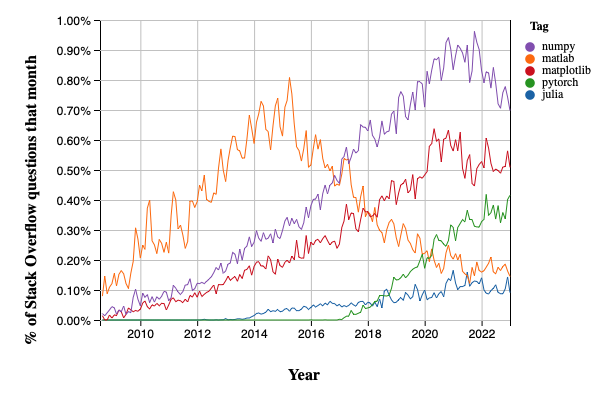
\includegraphics{python_vs_rest.png}}
       \end{center}
    \end{figure}

\end{frame}



\begin{frame}
    \frametitle{Trend 2: Low Level $\to$ High Level}
    
    \blue{Low level} 
    
    \begin{itemize}
        \item C/C++
        \item Fortran
        \item Assembly
    \end{itemize}

    \vspace{1em}

    \blue{High level } 

    \begin{itemize}
        \item Python
        \item Javascript
        \item PHP
    \end{itemize}

\end{frame}


\begin{frame}
    
    \blue{Low level languages} give us control 

    \begin{itemize}
        \item control CPU
        \item control memory
    \end{itemize}

    \vspace{0.5em}
    \vspace{0.5em}
    \vspace{0.5em}

    \blue{High level languages} give us 
    %
    \begin{itemize}
        \item abstraction
        \item automation
        \item flexibility, etc.
    \end{itemize}

\end{frame}




\begin{frame}[fragile]

    \Eg \brown{1 + 1} in assembly

    {\small
    \begin{minted}{as}
pushq   %rbp
movq    %rsp, %rbp
movl    $1, -12(%rbp)
movl    $1, -8(%rbp)
movl    -12(%rbp), %edx
movl    -8(%rbp), %eax
addl    %edx, %eax
movl    %eax, -4(%rbp)
movl    -4(%rbp), %eax
popq    %rbp
    \end{minted}
    }

\end{frame}


\begin{frame}[fragile]

    \Eg \brown{1 + 1} in C/C++

    {\small
    \begin{minted}{c}
#include <stdio.h>
int main() {
    int sum = 1 + 1;
    printf("1 + 1 = %d\n", sum);
    return 0;
}   
    \end{minted}
    }

\end{frame}

\begin{frame}[fragile]

    \Eg \brown{1 + 1} in Python

    {\small
    \begin{minted}{python}
sum = 1 + 1
print("1 + 1 = ", sum)
    \end{minted}
    }

\end{frame}



\begin{frame}

    Trade-Offs:

    \begin{figure}
       \begin{center}
        \scalebox{.36}{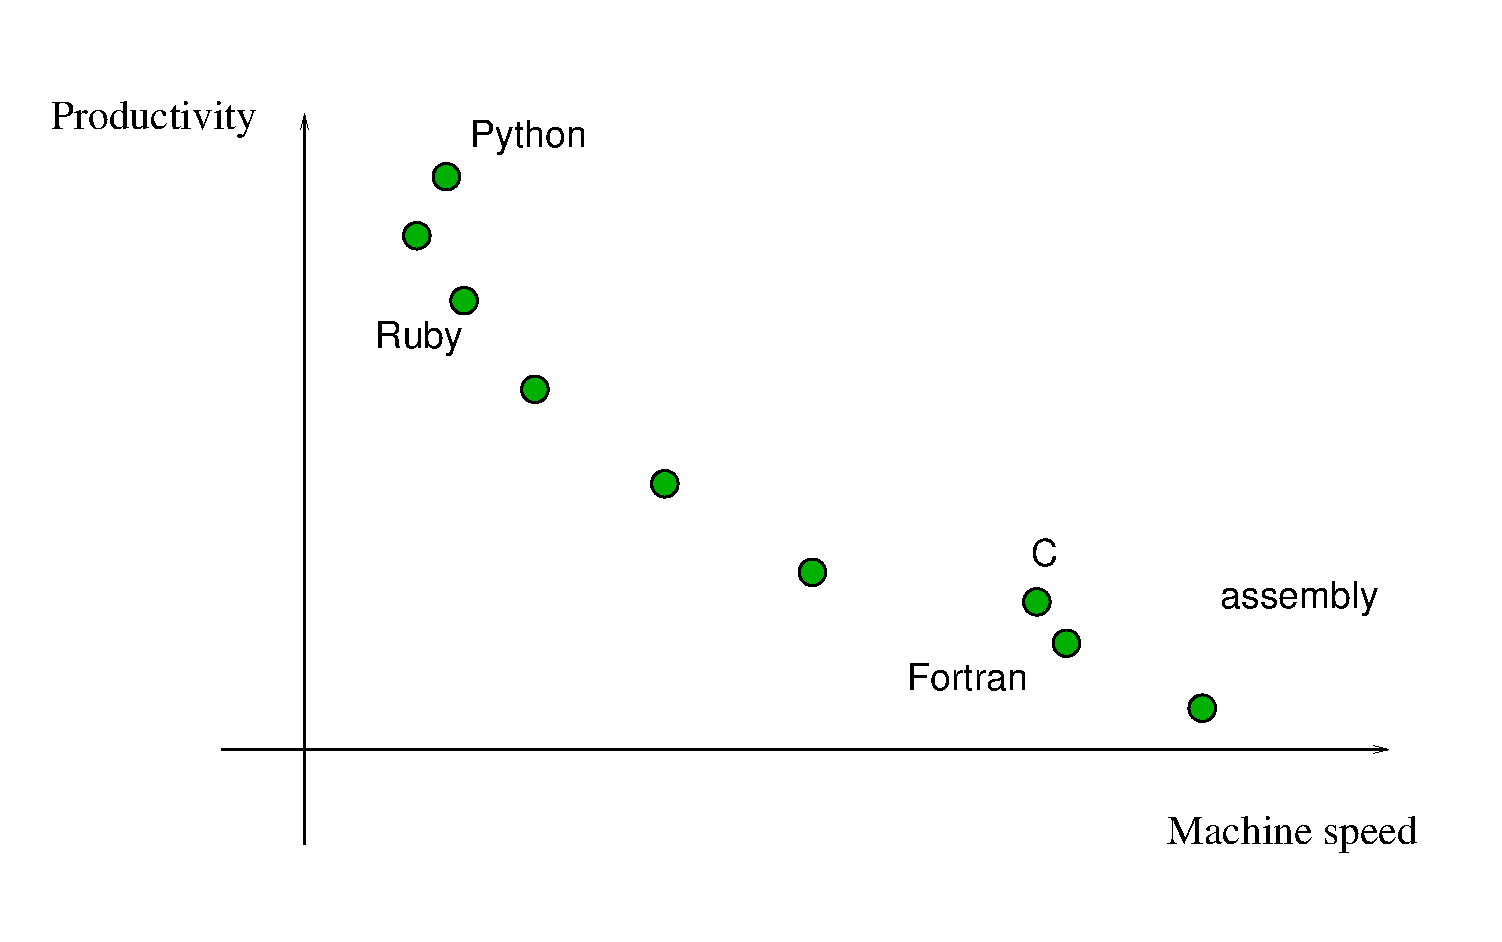
\includegraphics{tradeoff.pdf}}
       \end{center}
    \end{figure}

\end{frame}



\begin{frame}[fragile]

    \emp{But what about scientific computing?}
    
            \vspace{0.4em}
            \vspace{0.4em}
            \vspace{0.4em}

    Requirements:

    \begin{itemize}
        \item \underline{\green{Productive}} --- easy to read, write, debug, explore
            \vspace{0.4em}
            \vspace{0.4em}
            \vspace{0.4em}
        \item \underline{\green{Fast}} computations
    \end{itemize}

\end{frame}




\begin{frame}

    Trade-offs:

    \begin{figure}
       \begin{center}
        \scalebox{.36}{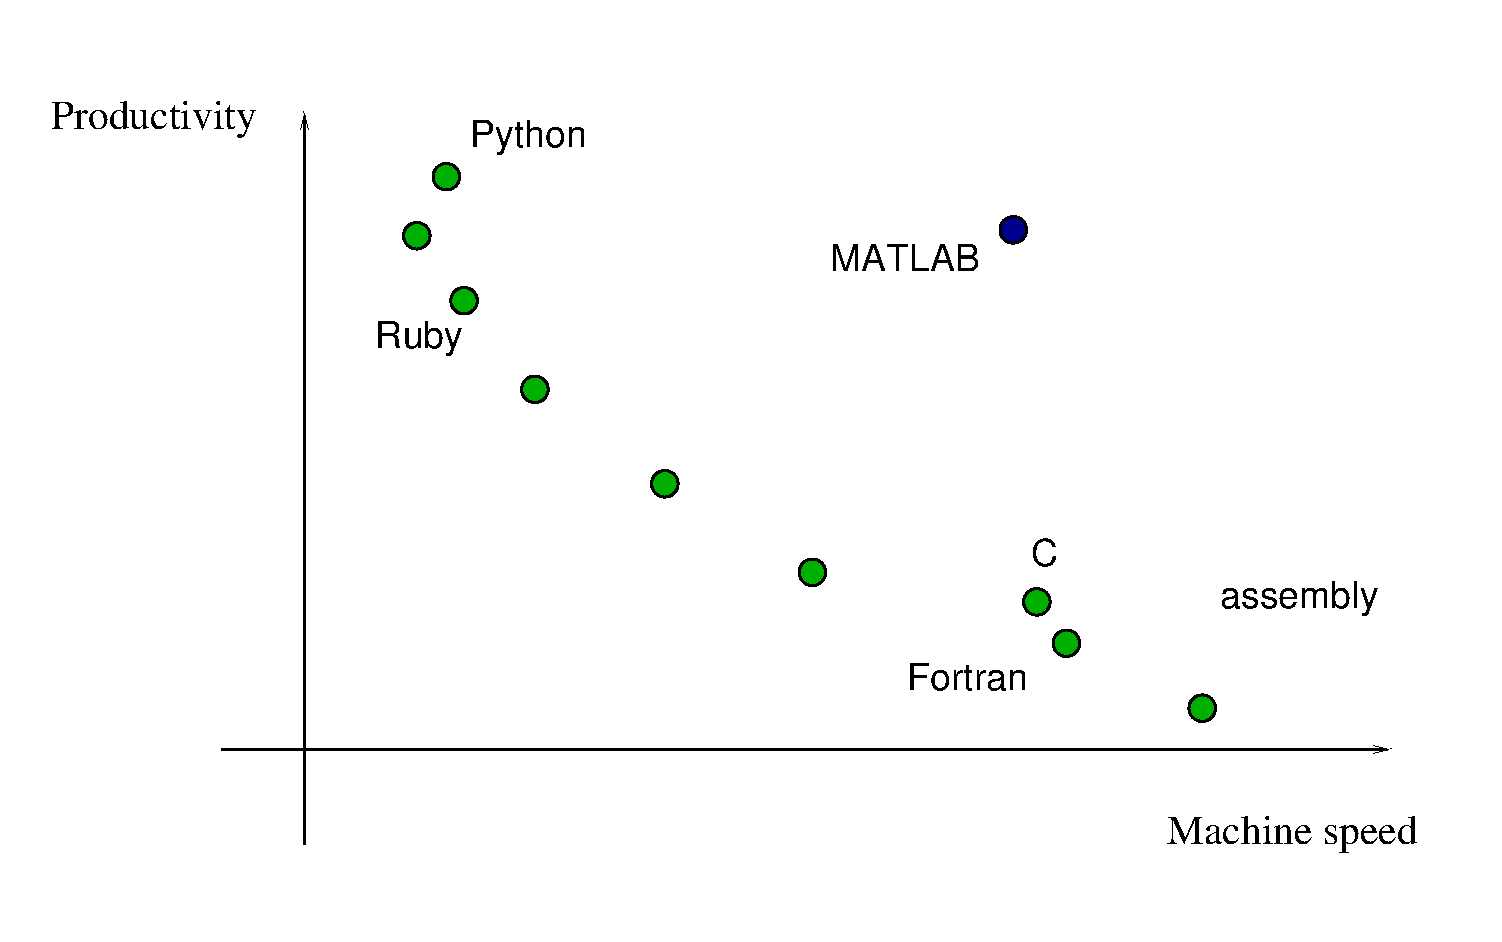
\includegraphics{tradeoff2.pdf}}
       \end{center}
    \end{figure}

\end{frame}


\begin{frame}

    Trade-offs:

    \begin{figure}
       \begin{center}
        \scalebox{.36}{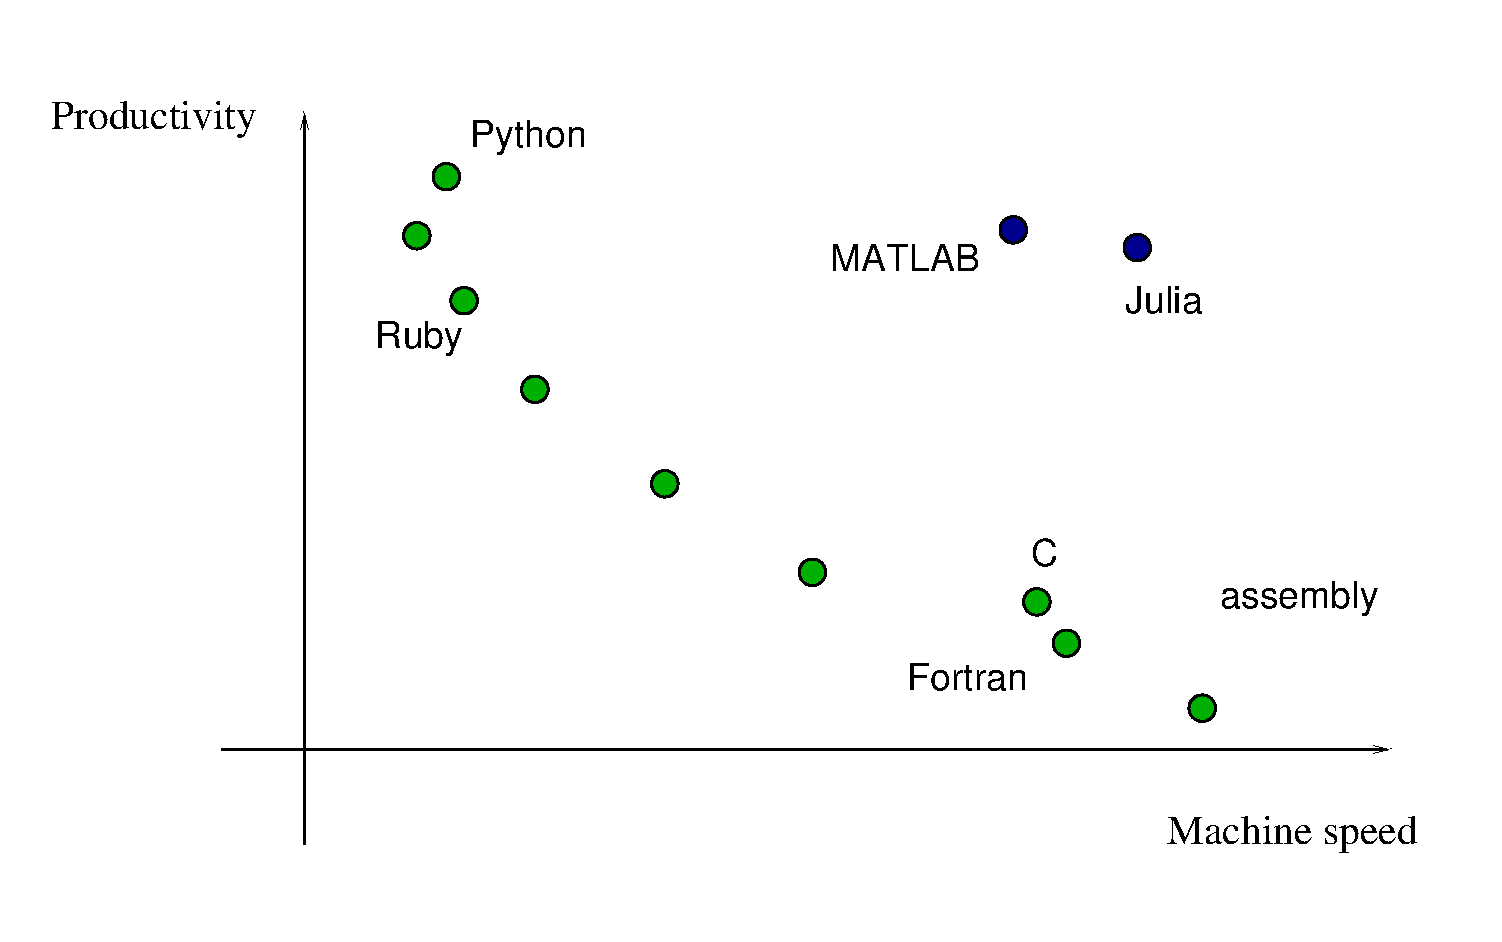
\includegraphics{tradeoff3.pdf}}
       \end{center}
    \end{figure}

\end{frame}


\begin{frame}

    Trade-offs:

    \begin{figure}
       \begin{center}
        \scalebox{.36}{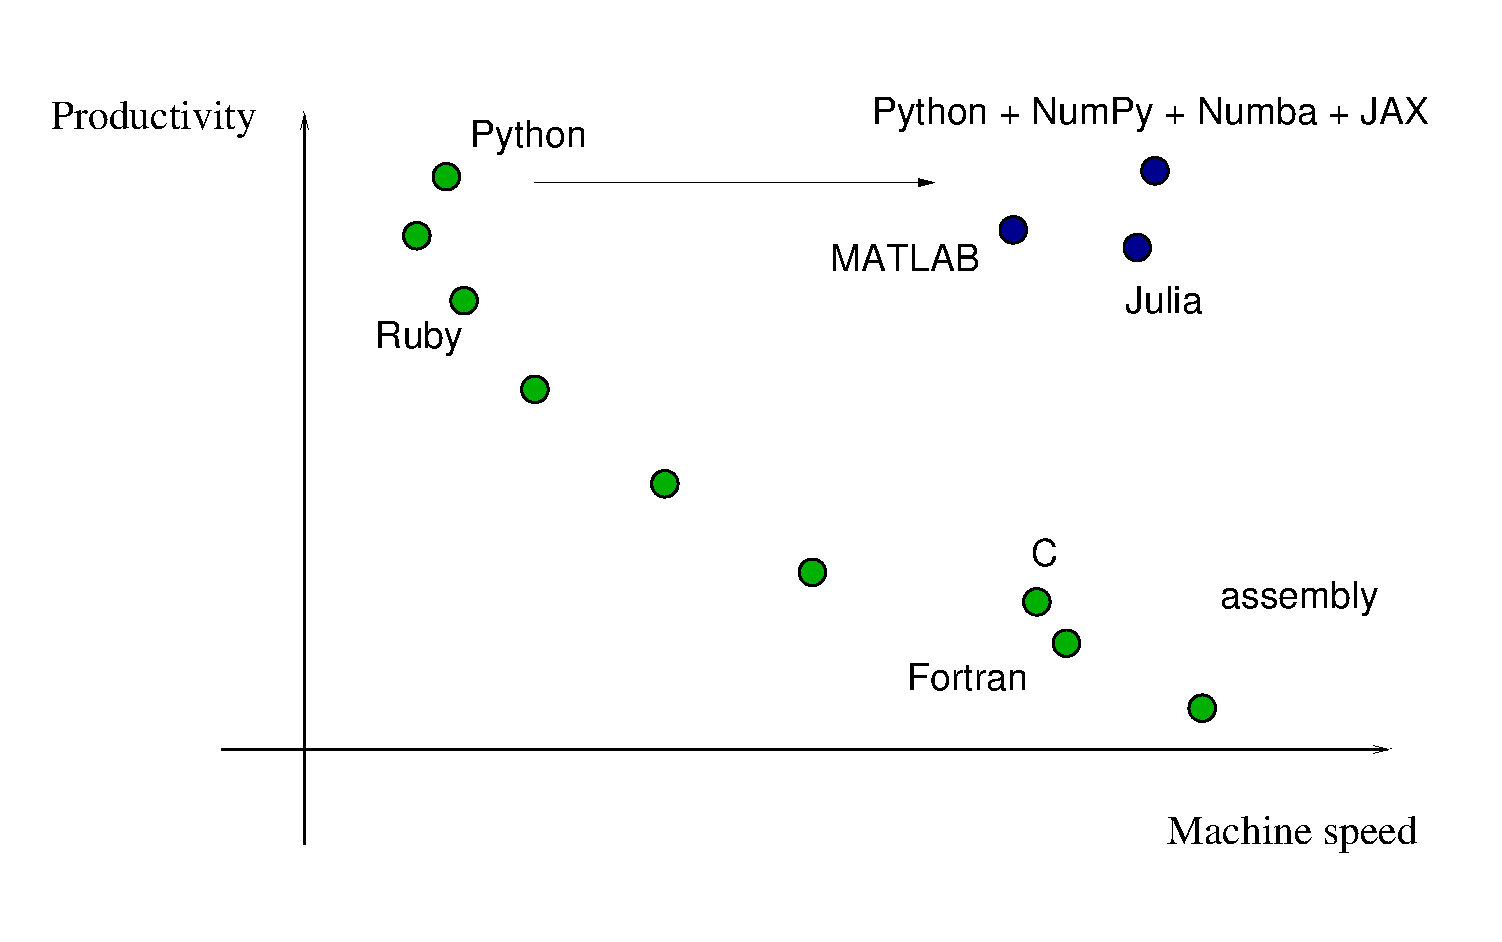
\includegraphics{tradeoff4.pdf}}
       \end{center}
    \end{figure}

\end{frame}



\begin{frame}

    \Eg What platforms/languages does OpenAI use?

        \vspace{0.5em}
    In order (according to  \href{https://github.com/openai}{repo stats}):

    \begin{enumerate}
        \item Python
        \item C/C++
        \item Javascript
        \item Jupyter notebooks
        \item Ruby
    \end{enumerate}

\end{frame}



%\section{Parallelization}

\begin{frame}
    \frametitle{Trend 3: Parallelization}

    CPU frequency (clock speed) growth is slowing

    \begin{figure}
       \begin{center}
        \scalebox{.22}{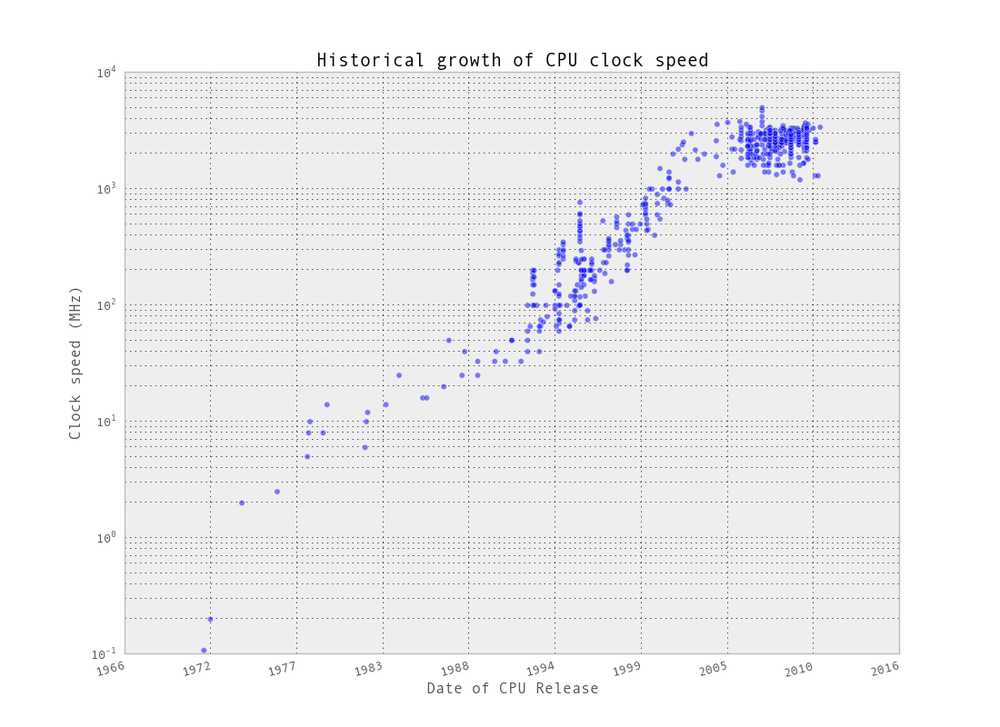
\includegraphics{processor_clock.png}}
       \end{center}
    \end{figure}

\end{frame}


\begin{frame}
    
    Chip makers have responded by developing multi-core processors

    \begin{figure}
       \begin{center}
        \scalebox{.2}{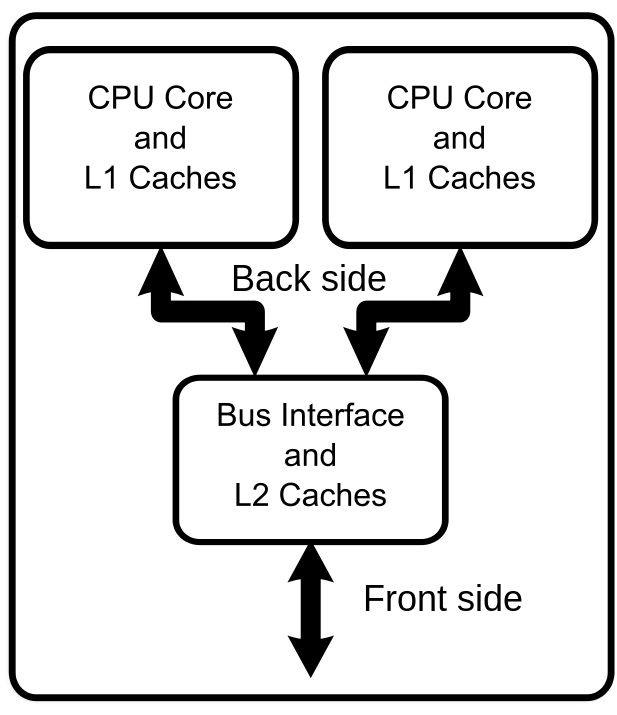
\includegraphics{dual_core.png}}
       \end{center}
    \end{figure}

    Source: Wikipedia


\end{frame}


\begin{frame}

    \navy{GPUs} are becoming increasingly important


    \begin{figure}
       \begin{center}
        \scalebox{.16}{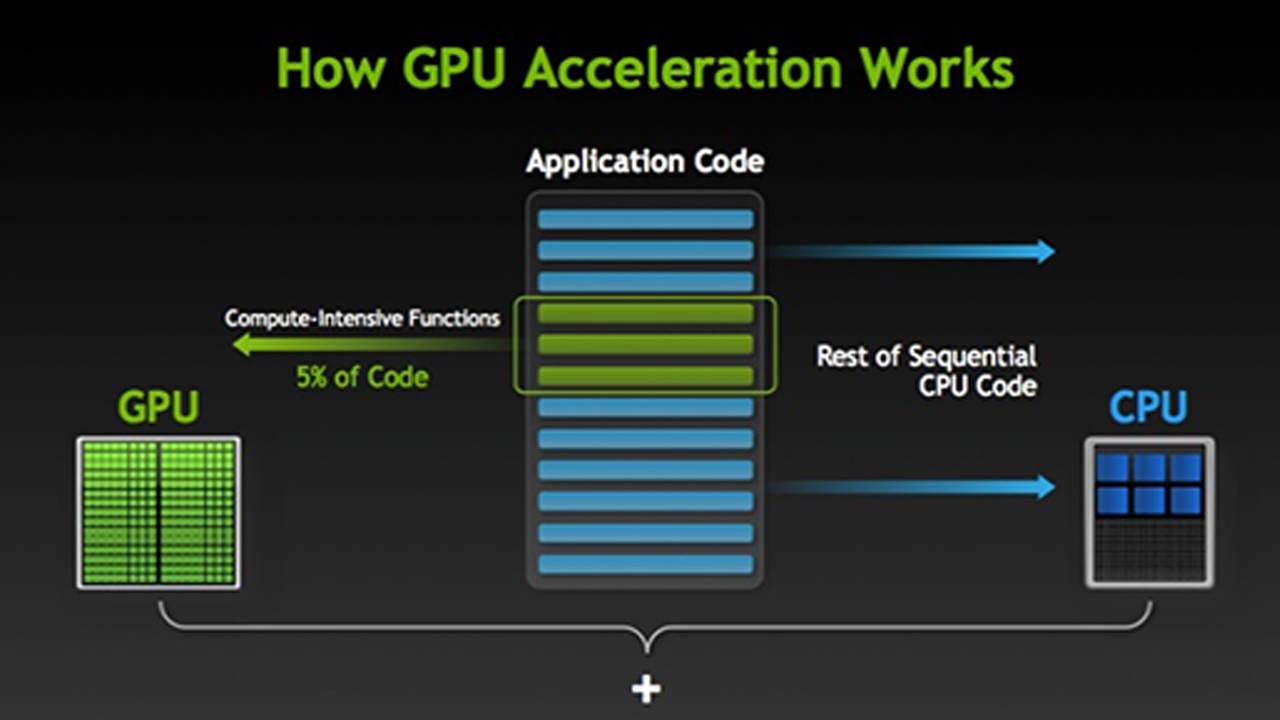
\includegraphics{gpu.jpg}}
       \end{center}
    \end{figure}

    \vspace{0.5em}

    Applications: machine learning, deep learning, etc.
    

\end{frame}



\begin{frame}
    \frametitle{Support for Parallelization}
    
    While scientific computing environments best support parallelization?

        \vspace{0.5em}
        \vspace{0.5em}
    %
    \begin{itemize}
        \item Most have some support
        \vspace{0.5em}
        \item but which make it easy to harness its power?
    \end{itemize}

    \vspace{0.5em}
    \vspace{0.5em}

    Current winner:
    %
    \begin{itemize}
        \item Google JAX (Python library)
            \vspace{0.5em}
    \end{itemize}

\end{frame}




\section{Which Language?}


\begin{frame}
    \frametitle{Which Language}


    How about R?
    \vspace{0.5em}

    \begin{itemize}
        \item Specialized to statistics
            \vspace{0.5em}
        \item Huge range of estimation routines
            \vspace{0.5em}
        \item Popular in academia 
            \vspace{0.5em}
        \item Loosing some ground to Python (AI, machine learning)
    \end{itemize}

\end{frame}


\begin{frame}
    \frametitle{Julia}

    Pros:
    
    \begin{itemize}
        \item Fast and elegant
            \vspace{0.5em}
        \item Many scientific routines
            \vspace{0.5em}
        \item Julia is written in Julia
    \end{itemize}

            \vspace{0.5em}
            \vspace{0.5em}
            \vspace{0.5em}
    Cons:
    
    \begin{itemize}
        \item Low rates of investment in some important libraries
    \end{itemize}

\end{frame}




\begin{frame}
    \frametitle{Python}
    
    \begin{itemize}
        \item Easy to learn, well designed
            \vspace{0.5em}
        \item Massive scientific ecosystem
            \vspace{0.5em}
        \item Heavily supported by big players
            \vspace{0.5em}
        \item Strong support for parallel computing
            \vspace{0.5em}
        \item Huge demand for tech-savvy Python programmers
    \end{itemize}


\end{frame}




\section{Set Up}





\begin{frame}
    \frametitle{Accessing Python}

    Option 1: \green{Via a service (remote option)}

    \begin{itemize}
        \item \url{https://colab.research.google.com}
    \end{itemize}

    \vspace{1em}

    Option 2: \green{Local install (Python + scientific libs)}
    
    \begin{itemize}
        \item Install Anaconda from {\footnotesize \url{https://www.anaconda.com/}}
        \vspace{1em}
            \begin{itemize}
                \item Select latest version 
            \end{itemize}
        \vspace{1em}
        \item Not plain vanilla Python
    \end{itemize}




\end{frame}



\begin{frame}
    \frametitle{How to Interact with Python?}

    Many options:

    \begin{itemize}
        \item \emp{write} with VS Code / Emacs / Vim
            \vspace{0.5em}
        \item \emp{run} with base Python, IPython, etc.
    \end{itemize}

            \vspace{0.5em}
            \vspace{0.5em}
            \vspace{0.5em}
        Or do both with \emp{Jupyter notebooks / Jupyter lab}

            \vspace{0.5em}
    \begin{itemize}
        \item for simplicity we focus only on the last option
    \end{itemize}

\end{frame}


\begin{frame}
    \frametitle{Jupyter Notebooks}

    A browser based interface to Python / Julia / R / etc.


    \vspace{2em}

    \begin{itemize}
        \item Search for \texttt{jupyter notebook}
    \end{itemize}

    \vspace{2em}

    Useful for:

    \begin{itemize}
        \item getting started
        \item exploring ideas
    \end{itemize}

\end{frame}



\begin{frame}
    \frametitle{Working with Notebooks}

    \begin{itemize}
        \item Entry and execution
    \vspace{1em}
        \item Markdown
    \vspace{1em}
        \item Getting help
    \vspace{1em}
        \item Copy paste
    \vspace{1em}
        \item Edit and command mode
    \end{itemize}

\end{frame}



\begin{frame}
    \frametitle{RA Work}

    We and other academics are looking for talented RAs

            \vspace{0.5em}
    Ideal skills

    \begin{itemize}
        \item git and GitHub
            \vspace{0.5em}
        \item Python
            \vspace{0.5em}
        \item scientific libraries
            \vspace{0.5em}
        \item maths
            \vspace{0.5em}
        \item stats
            \vspace{0.5em}
        \item economics
    \end{itemize}

\end{frame}







\end{document}


